\documentclass{article}
\usepackage{geometry}
\geometry{
	a4paper,
	%total={170mm,257mm},
	left=20mm,
	top=30mm,
}

\usepackage{fancyhdr}
\usepackage{tikz}
\usepackage{hyperref}
\usepackage{graphicx}
\usepackage{hyperref}
\usepackage{mdframed}
\usepackage{listings} % Include the listings package
\usepackage{xcolor}   % to define your own colors
\usepackage{subcaption}

\bibliographystyle{unsrt}
\bibliography{references}


\newmdenv[
linecolor=blue, % Color of the border line
backgroundcolor=gray!20, % Background color; "gray!20" means "20% gray"
frametitle=Note, % Title of the frame, delete this line if you don't want a title
skipabove=\baselineskip, % Space above the frame
skipbelow=\baselineskip, % Space below the frame
]{mynote}

% code-snippets:
% Define the color styles you wish to use in the document for the Python syntax highlighting
\lstdefinestyle{mystyle}{
	backgroundcolor=\color{white},   % choose the background color; you must add \usepackage{color} or \usepackage{xcolor}
	commentstyle=\color{green},
	keywordstyle=\color{blue},
	numberstyle=\tiny\color{gray},
	stringstyle=\color{red},
	basicstyle=\ttfamily\footnotesize,
	breakatwhitespace=false,         
	breaklines=true,                 
	captionpos=b,                    
	keepspaces=true,                 
	numbers=left,                    
	numbersep=5pt,                  
	showspaces=false,                
	showstringspaces=false,
	showtabs=false,                  
	tabsize=2
}

\lstset{style=mystyle} % Apply your style globally to the document


\newcommand{\LVA}{Reverse Engineering}
\newcommand{\LVAKURZ}{REV3}
\newcommand{\SEMESTER}{WS 2023/2024}
\newcommand{\UELABEL}{UE 02}
\newcommand{\UETITLE}{Statische Analyse}
\newcommand{\AUTHOR}{Jakob Mayr}


\title{\vspace{5cm} \LVA\ (\LVAKURZ)\\ \vspace{1cm} \textbf{\UELABEL\ -- \UETITLE\ -- Protokoll} \vspace{2.5cm}}
\author{\AUTHOR}
\date{\SEMESTER}

\begin{document}
	
	\pagestyle{fancy}
	
	\maketitle
	
	\tikz [remember picture, overlay] %
	\node [shift={(3.7cm,-4cm)}] at (current page.north west) %
	[anchor=north west] %
	{
\includegraphics{fhooe_logo.jpg}};
	
	\tikz [remember picture, overlay] %
	\node [shift={(10cm,-4.8cm)}] at (current page.north west) %
	[anchor=north west] %
	{
\includegraphics{si_logo.jpg}};
	
	%\tikz [remember picture, overlay] %
	%\node [shift={(7.2cm,-11.65cm)}] at (current page.north west) %
	%[anchor=north west] %
	%{\includegraphics[scale=0.12]{./img/star_wars_logo_no_background.png}};
	%
	%\pagebreak
	
	\fancyhf{}
	\fancyhead[L]{\LVA\ (\LVAKURZ)}
	\fancyhead[C]{\UELABEL}
	\fancyhead[R]{\SEMESTER}
	\fancyfoot[L]{Seite \thepage\ von \pageref{LastPage}}
	\fancyfoot[R]{\AUTHOR}
	
	\section{Einleitung}
	...\\
	
	\pagebreak
	
	\section{Aufgabe 1 - Statische Analyse Windows}
	\subsection{create file}
		\begin{lstlisting}[language=c]
		#include <stdio.h>
		
		int main() {
			printf("infected");
			return = 0;
		}
	\end{lstlisting}
	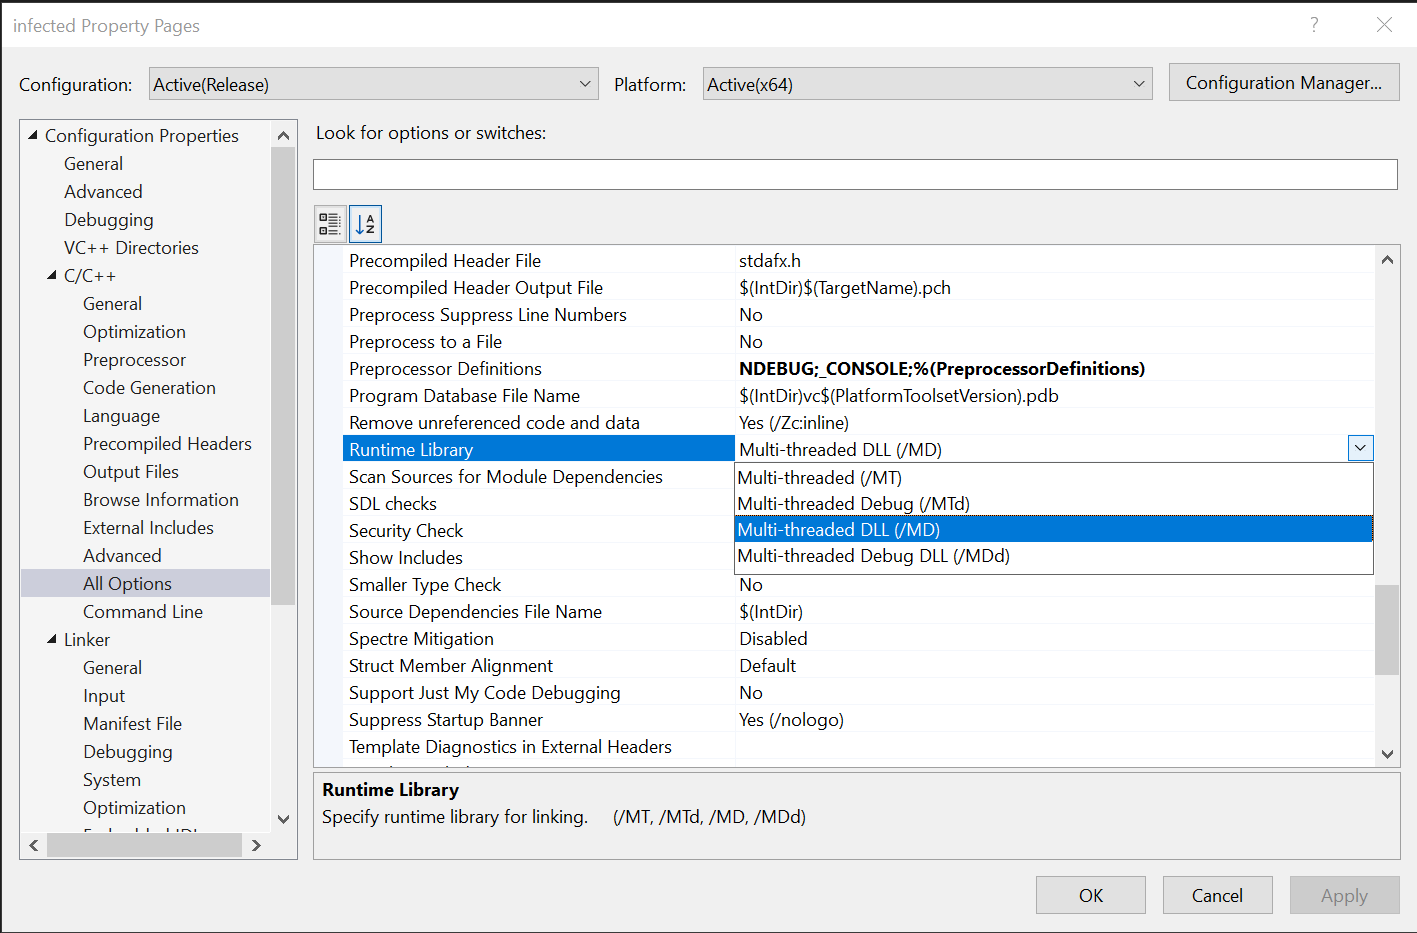
\includegraphics[width=0.7\linewidth]{pictures/1. setting runtime library.png}\\
	\\
	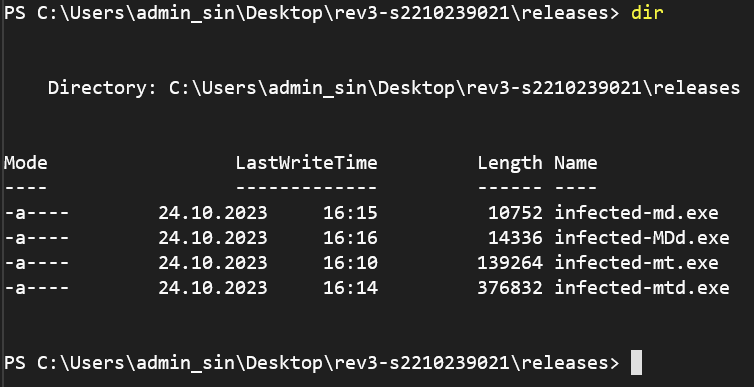
\includegraphics[width=0.5\linewidth]{pictures/1. all files.png}\\
	
	\pagebreak
	
	\subsection{dumpbin}
	\begin{figure}[htp]
		\centering
		\begin{subfigure}[b]{0.45\textwidth}
			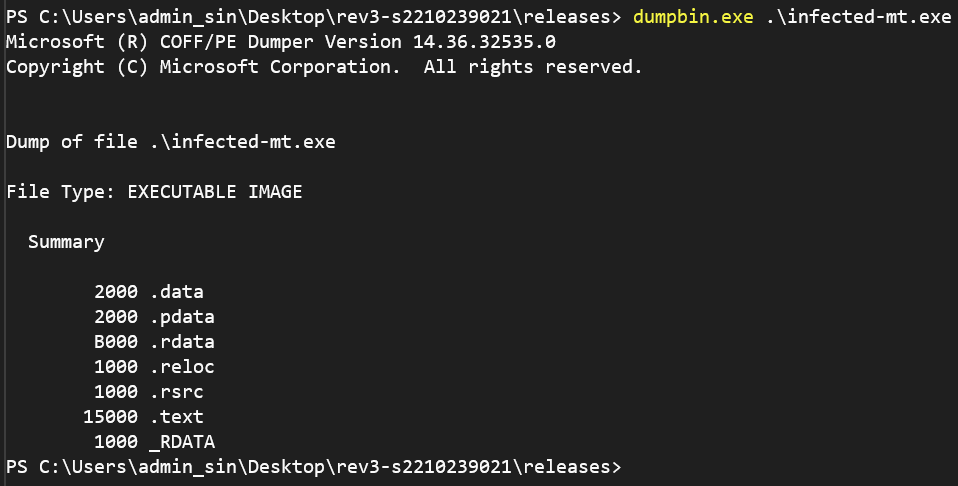
\includegraphics[width=\textwidth]{pictures/1. dumpbin mt.png}
			\caption{dumpbin mt-file}
			\label{fig:image1}
		\end{subfigure}
		\hfill
		\begin{subfigure}[b]{0.45\textwidth}
			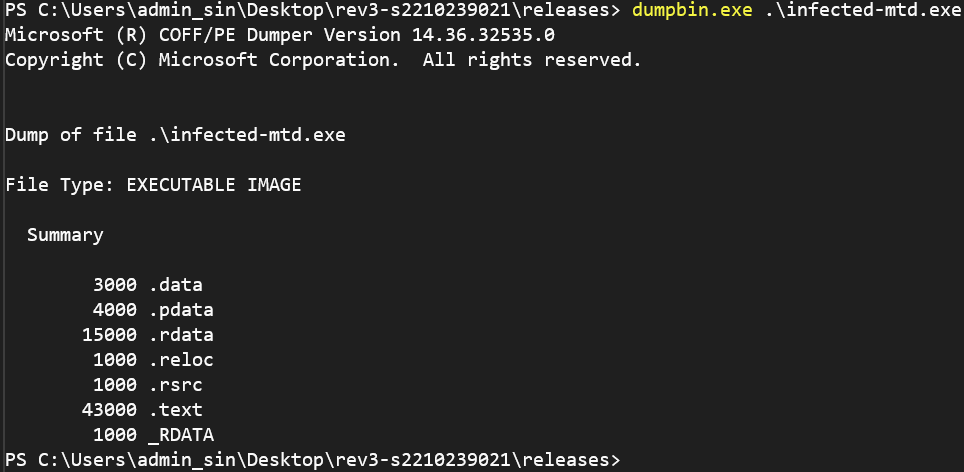
\includegraphics[width=\textwidth]{pictures/1. dumpbin mtd.png}
			\caption{dumpbin mtd-file}
			\label{fig:image2}
		\end{subfigure}
		
		\vspace{10pt} % Adjust to your liking
		
		\begin{subfigure}[b]{0.45\textwidth}
			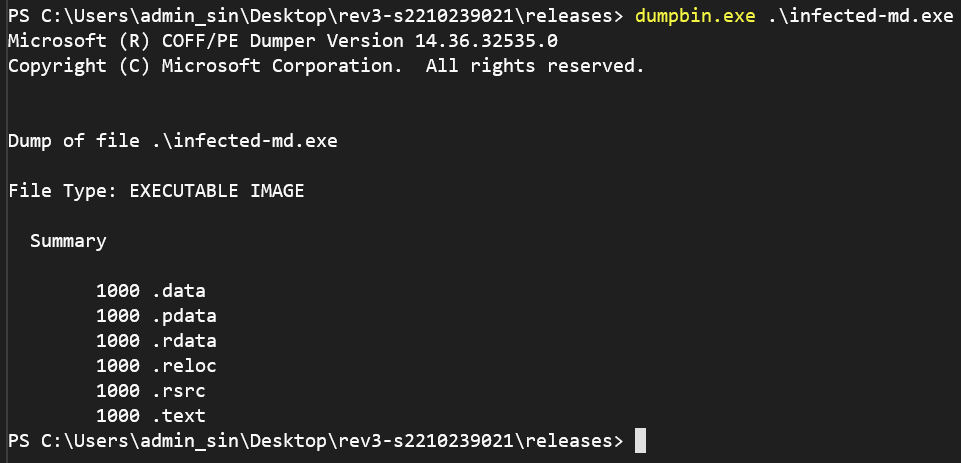
\includegraphics[width=\textwidth]{pictures/1. dumpbin md.png}
			\caption{dumpbin md-file}
			\label{fig:image3}
		\end{subfigure}
		\hfill
		\begin{subfigure}[b]{0.45\textwidth}
			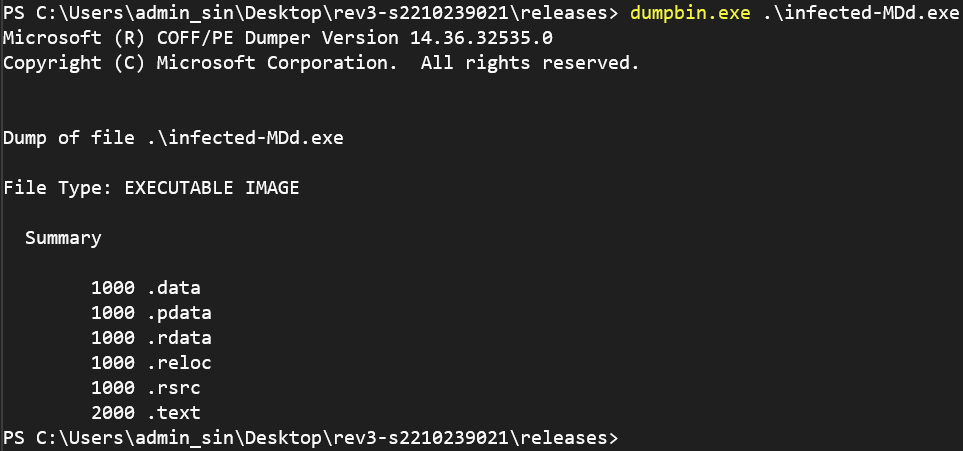
\includegraphics[width=\textwidth]{pictures/1. dumpbin mdd.png}
			\caption{dumpbin mdd-file}
			\label{fig:image4}
		\end{subfigure}
		\caption{All infected.exe files analysed with dumpbin}
		\label{fig:grid}
	\end{figure}
	
	\pagebreak
	
	\subsection{strings}
	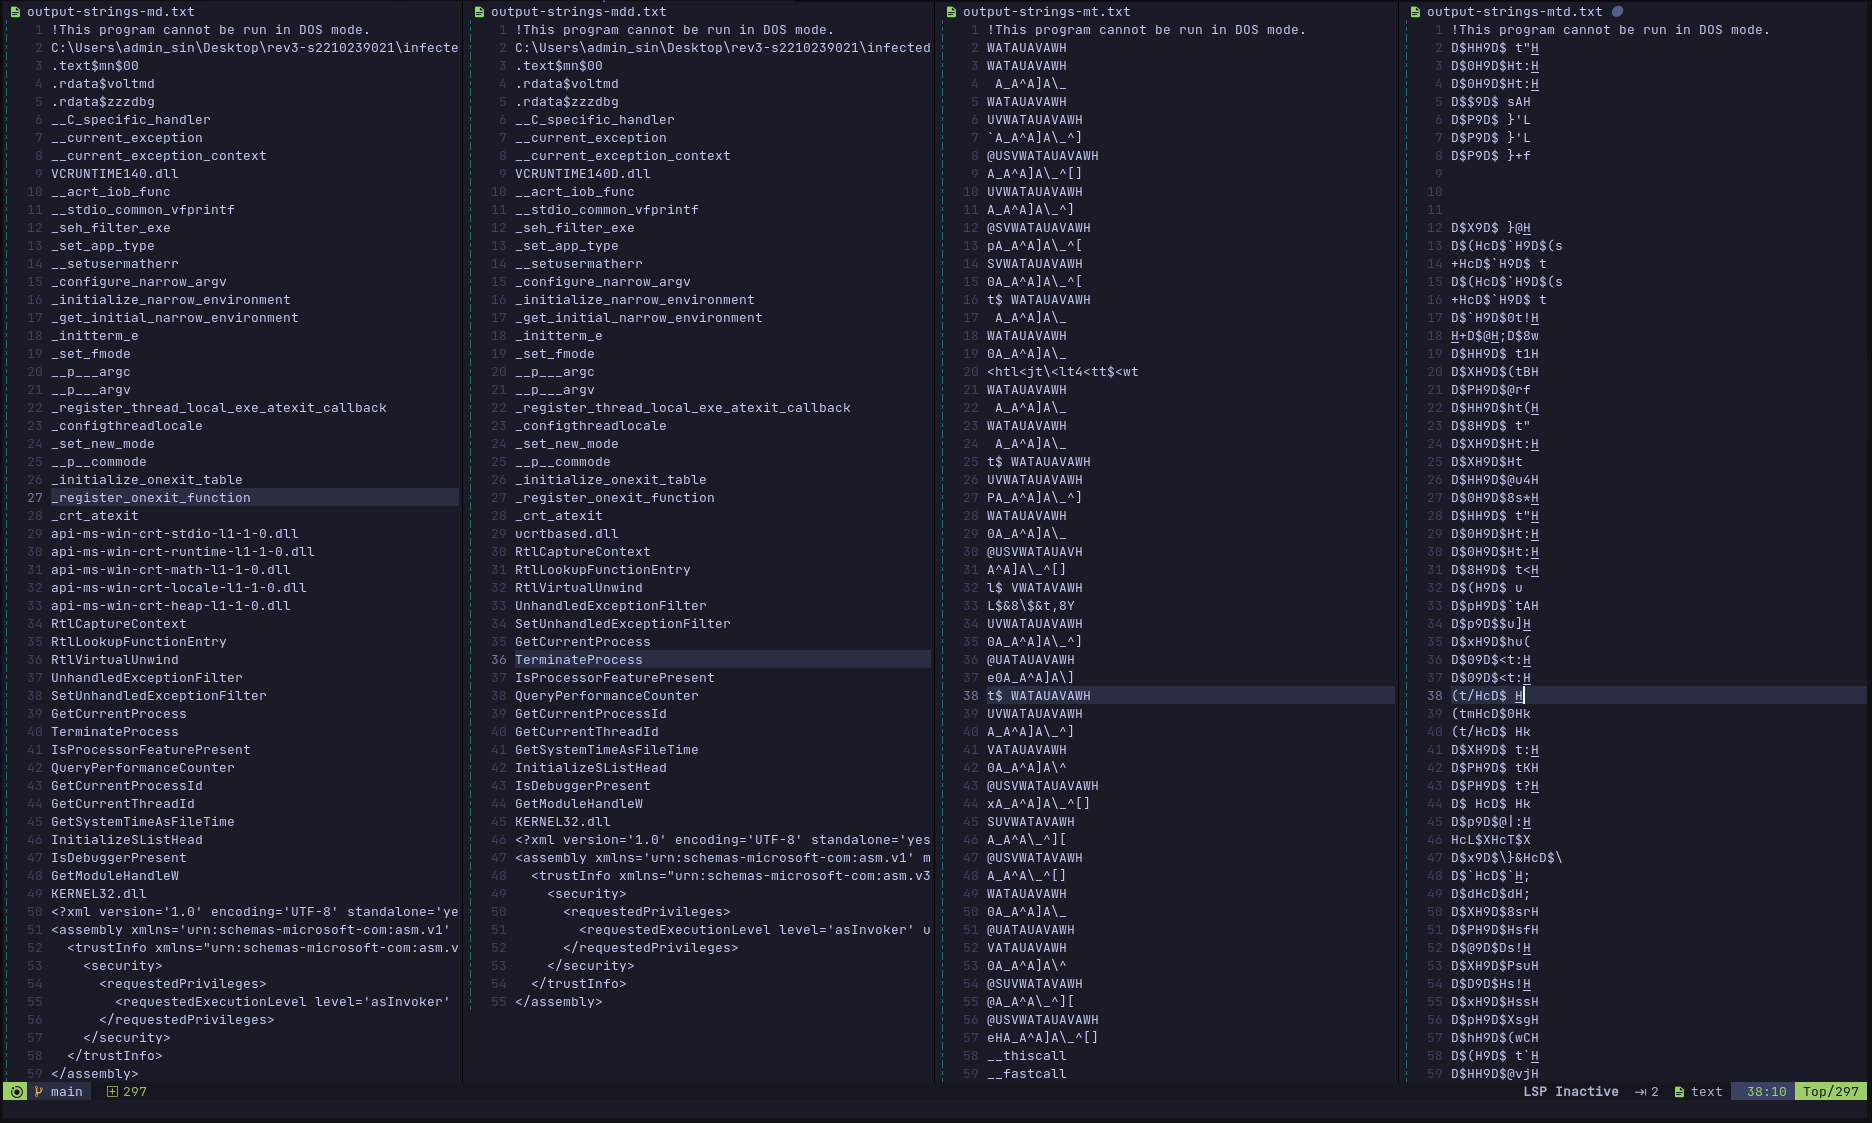
\includegraphics[width=1\linewidth]{pictures/1. strings from all files}\\
	\\
	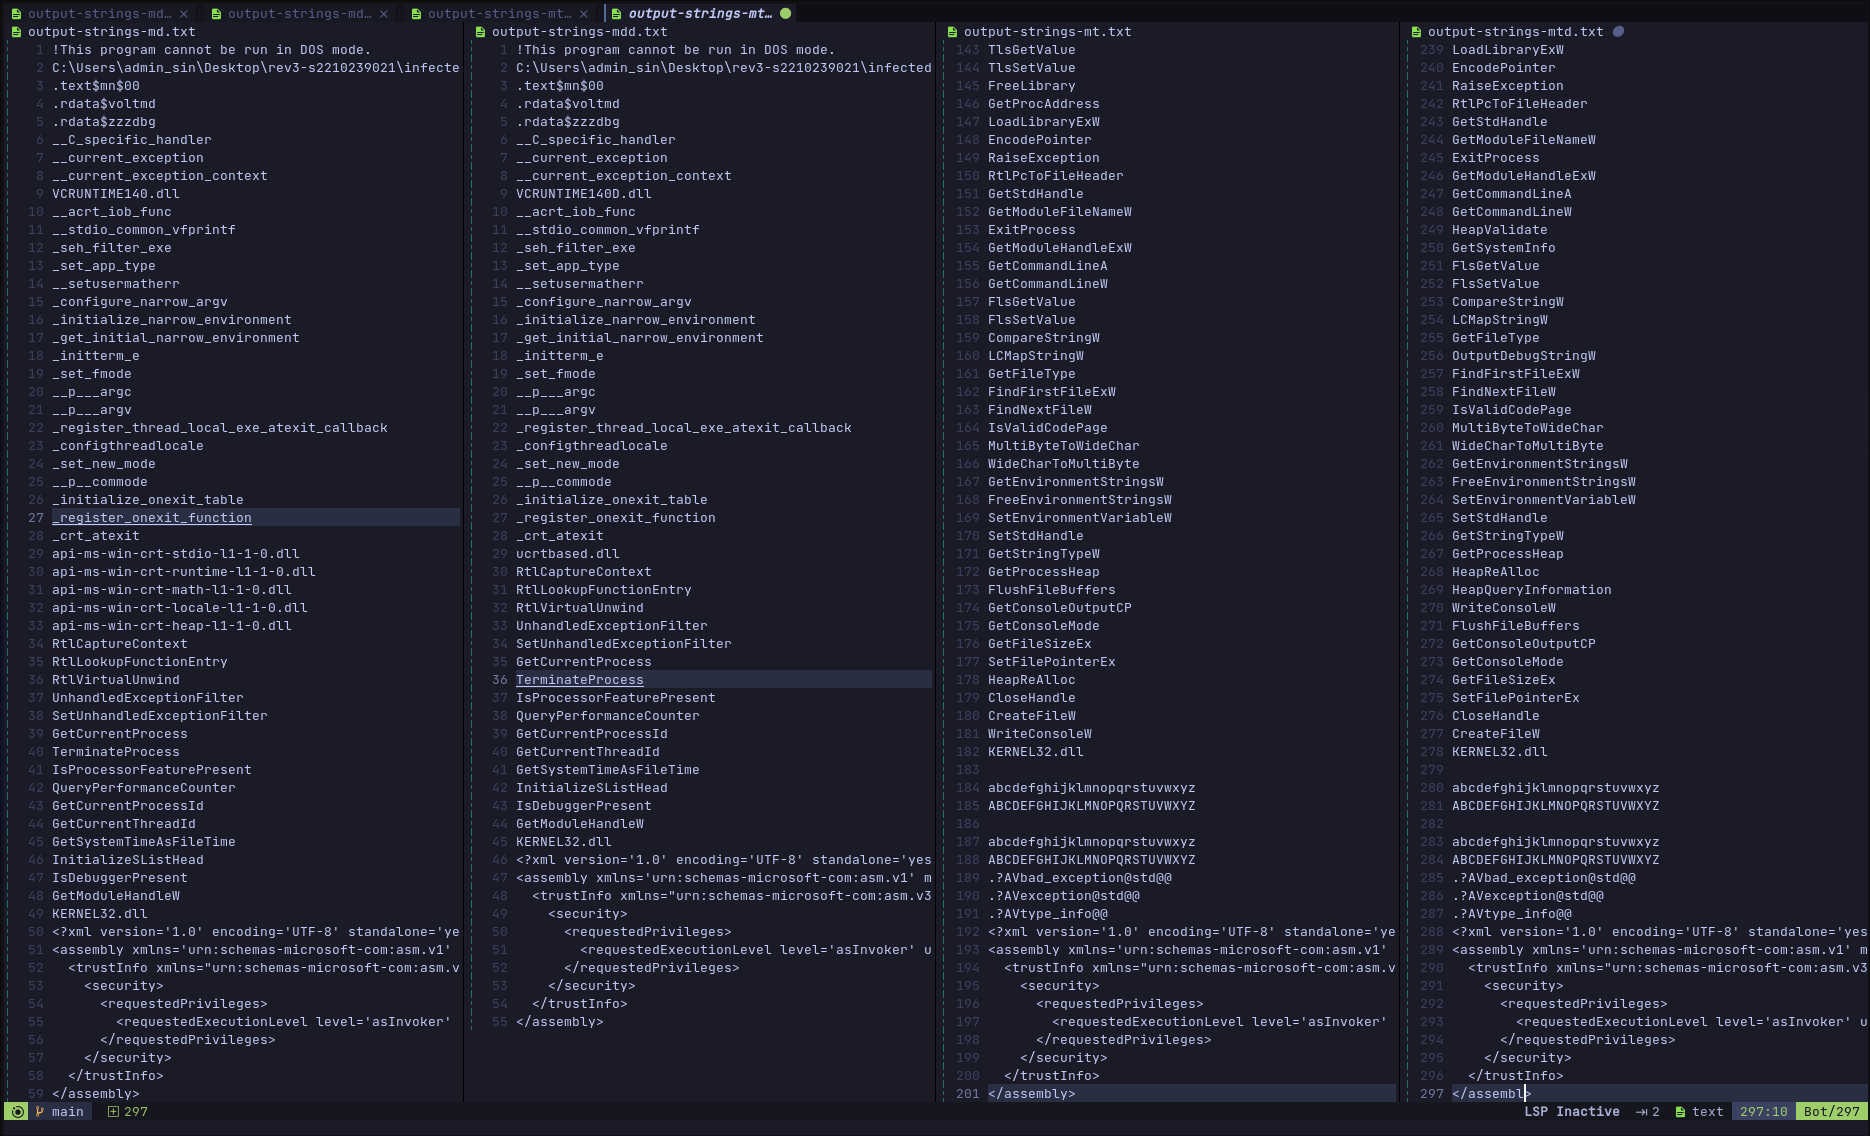
\includegraphics[width=1\linewidth]{pictures/1. strings from all files.2}\\
	
	
	\pagebreak
	
	\section{2. Aufgabe - Statische Analyse Linux}
	\subsection{create file}
	Gleicher code wie zuvor:\\
	\begin{lstlisting}[language=c]
		#include <stdio.h>
		
		int main() {
			printf("infected");
			return = 0;
		}
	\end{lstlisting}
	Kompilieren und auflisten der Executables:\\
	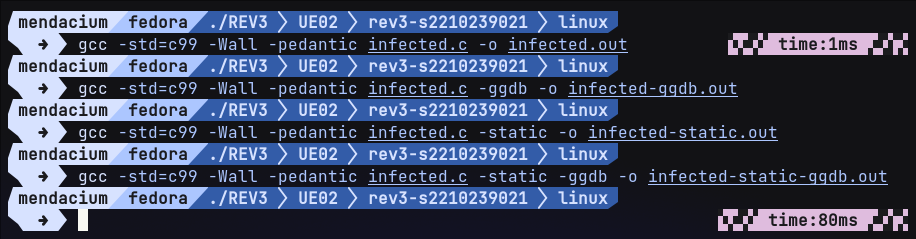
\includegraphics[width=0.7\linewidth]{pictures/2. compile files}\\
	\\
	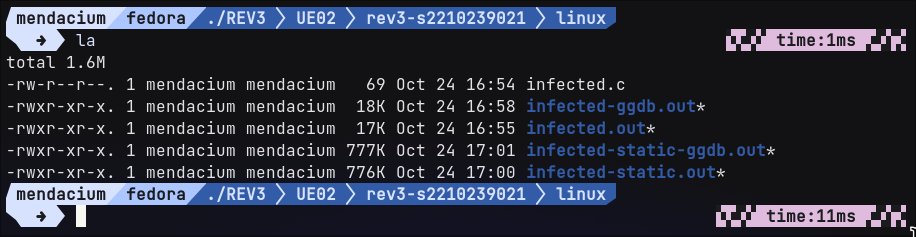
\includegraphics[width=0.5\linewidth]{pictures/2. all files}\\
	
	\pagebreak
	
	
	\begin{thebibliography}{9}
		
		\bibitem{radare2}
		\emph{The Official Radare2 Book},
		[Online; abgerufen im Oktober 2023],
		\url{https://book.rada.re/}.
		
	\end{thebibliography}
	
	
	\label{LastPage}
	
\end{document}